\documentclass[11pt, oneside]{article}   	% use "amsart" instead of "article" for AMSLaTeX format
\usepackage{geometry}                		% See geometry.pdf to learn the layout options. There are lots.
\geometry{letterpaper}                   		% ... or a4paper or a5paper or ... 
%\geometry{landscape}                		% Activate for rotated page geometry
%\usepackage[parfill]{parskip}    		% Activate to begin paragraphs with an empty line rather than an indent
\usepackage{graphicx}				% Use pdf, png, jpg, or eps§ with pdflatex; use eps in DVI mode
								% TeX will automatically convert eps --> pdf in pdflatex		
\usepackage{amssymb}

%SetFonts
\graphicspath{ {./images/} }
%SetFonts

\usepackage{caption}
\captionsetup[figure]{labelformat=empty}%
\usepackage{subcaption} 

\title{Crittografia}
%\author{The Author}
%\date{}							% Activate to display a given date or no date
\usepackage{float}
\begin{document}
\maketitle
%\section{}
%\subsection{}
Mercoledi: 13 - 14.30, 
Venerdì: 13 - 14.30\\
Modalità d'esame: orale - 16233\\
Programma:
\begin{itemize}
\item Accenni storici
\item Cifrario simmetrico con una chiave
\item Cifrario asimmetrico con due chiavi, una per aprire una per chiudere
\item Funzioni hash
\end{itemize}

In un cifrario simmetrico, la chiave di enconding è uguale alla chiave di decoding; nel cifrario asimmetrico le chiavi di enconding e decoding sono differenti.\\
Dato un mittente A, ed un ricevente B, il mittente A cifra il plain text in cypher text utilizzando le chiavi di enconding. Il cypher text viene trasmesso nel canale di comunicazione, che verrà poi passerà nel processo di decoding da parte di B, per ricavare nuovamente il plain text iniziale. \\
Scenari di attacco:\\
1) Cyphertext only \\ 
2) Known plaintext \\
3) Chosen plaintext \\
4) Chosen cyphertext \\\\
- I cifrari simmetrico vengono utilizzate per cifrari grosse quantità di dati (eg. testo, \emph{des e aes})\\
- I cifrari asimmetrici vengono utilizzati per cifrare piccole quantità di dati (eg. pw, \emph{rsa, elgamal})\\
- Le tecniche steganografiche sono tecniche di offuscazione del messaggio\\\\
Principio di Kerkhoff: un cifrario è forte sse l'attaccante conosce tutto tranne che la chiave. \emph{Brutalmente: se un cifrario rimane pubblico per 30 anni, ma non viene bucato, vuol dire che è resiliente.}\\\\
4 proprietà delle funzioni crittografiche:\\
- Confidenzialità: ottenuta attraverso l'operazione di cifratura prima della spedizione\\
- Integrità dei dati: applicando una funzione crittografica, se il risultato è medesimo nel caso del mittente e del destinatario la cifratura è considerata integro (hashing functions)\\
- Autenticazione: garantire che solo gli interessati siano in grado di accedere alle informazioni\\
- Non ripudio:  l'autore di una dichiarazione non potrà negare la paternità e la validità della dichiarazione stessa\\\\
Cifrari storici:\\\\
\textbf{Cifrario di Cesare} \\
Basato sulla traslazione delle lettere, dato un k trasliamo l'alfabeto di k valori\\\\
\textbf{Quadrato di Polibio} \\
Viene creato una matrice, si inseriscono le lettere all'interno della matrice e per ogni corrispondenza si prende la coppia colonna riga. Il cyphertext è grande 2x il plaintext. Il problema di questo cifrario è che ha punti fissi. \\
Un approccio migliore è passare da espressioni \(y = x + k \) a \(y = \alpha x + \beta \) con \(\alpha \neq 0   , \beta \neq 0 \)\\Per ricavare un valore dobbiamo fare \((y-\beta)/\alpha = x\). \\E' inoltre importante che MCD($\alpha, 26)$ = 1 ovvero che $\alpha$ sia invertibile, e che $\alpha$ e 26 siano \emph{coprimi}; il numero totale di chiavi possibili è $12 * 26$.\\\\
Come attacchiamo i crittosistemi affini? Andiamo ad analizzare il le frequenze. \\Dato il teorema di Kerkhoff l'attaccante conosce tutte le informazioni riguardo il cifrario, ma non la chiave.In italiano le lettere che compaiono di più sono E (che compare in media 11,79 \%), la A (11,74\%), la I (11,28 \%) etc.\\ Più il testo è lungo, più possiamo essere certi della corrispondenza (maggiore il campione, migliore l'approssimazione). Il problema del cifrario affine è quindi che data una lettera, la corrispondenza cifrata è sempre la stessa.\\\\
\textbf{Quadrato di Vigenère}
\begin{figure} [H]
\begin{center}
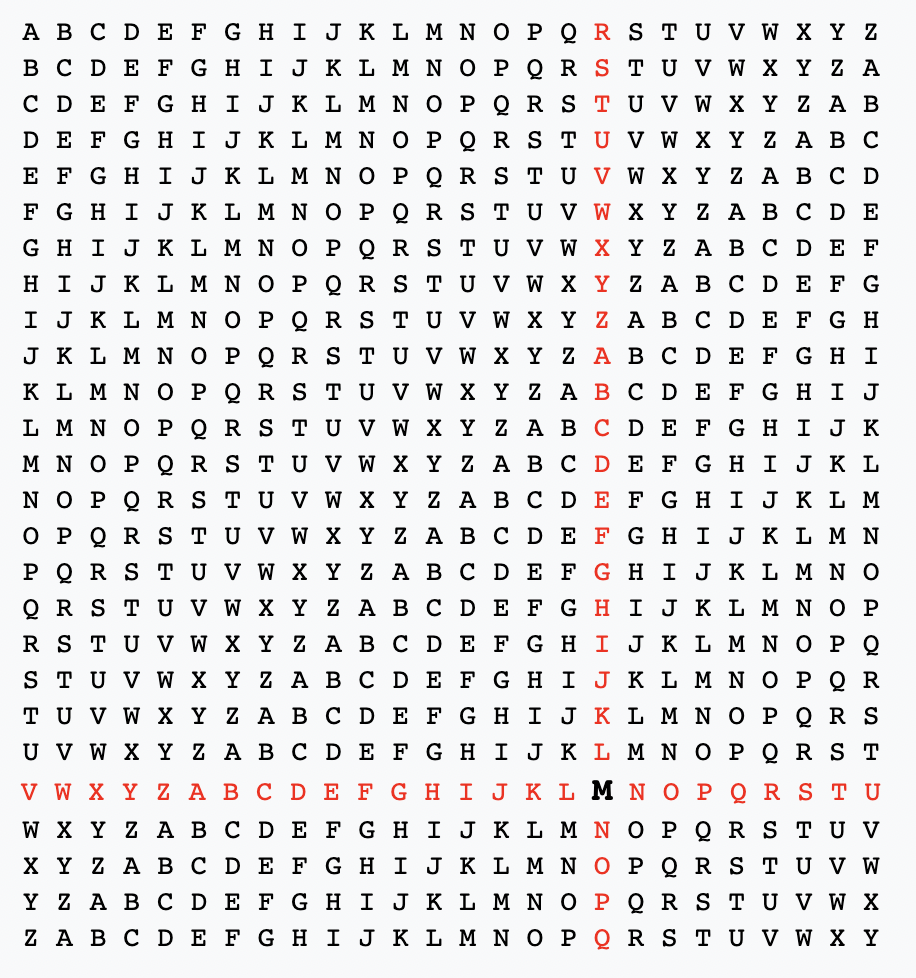
\includegraphics[scale=0.4]{vig}
\caption{codifica della lettera R con chiave V}
\end{center}
\end{figure}
Viene introdotta una chiave (parola), concordata tra mittente e destinatario. La chiave è ripetuta \emph{n} volte fino a ricavare una corrispondenza 1-1 con il messaggio da cifrare. In questo modo le stesse lettere hanno potenzialmente più corrispondenze. Per ricavare le singole lettere andiamo a ricavare la corrispondenza con colonna \(Cyphertext_i = (Plaintext_i, Chiave_i)\)
\begin{center}
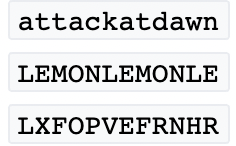
\includegraphics[scale=0.7]{chiave}
\end{center}
Come attacchiamo questo cifrario? Il metodo più famoso è il metodo di Kasiski\\
Attraverso \emph{l'analisi di Kasiski} possiamo sfruttare il fatto che alcune parole, per probabilità, vengono cifrate con le stesse lettere. Questo ci permette di trovare gruppi ripetuti nel \emph{cyphertext}.
\begin{center}
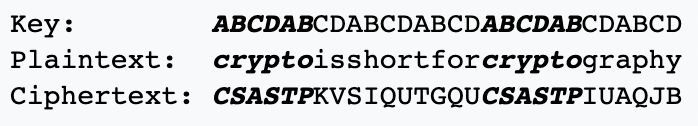
\includegraphics[scale=0.7]{freq}
\end{center}
Una volta identificati questi gruppetti, li raccogliamo e possiamo essere certi che questi sottoinsieme saranno un divisore della chiave. Possiamo quindi effettuare un'analisi di frequenza su queste, più lunga il testo, migliore sarà la precisione dell'analisi di frequenza.\\\\
Una variante è il cifrario di Cardano, in cui la chiave è inserita prima del crittotesto, tecnica molto vulnerabile in quanto è l'attaccante deve solo indovinare la lunghezza.\\\\
\textbf{Playfair cipher}
Il cifrario è basato su una matrice 5x5 (essendo l'alfabeto di 26, una lettera ha una corrispondenza con un'altra, solitamente i con j) in cui vengono inserite le lettere. La chiave è scelta, può essere una parola. Le lettere sono inserite saltando i doppioni, mettendo in testa la chiave.\\
\begin{center}
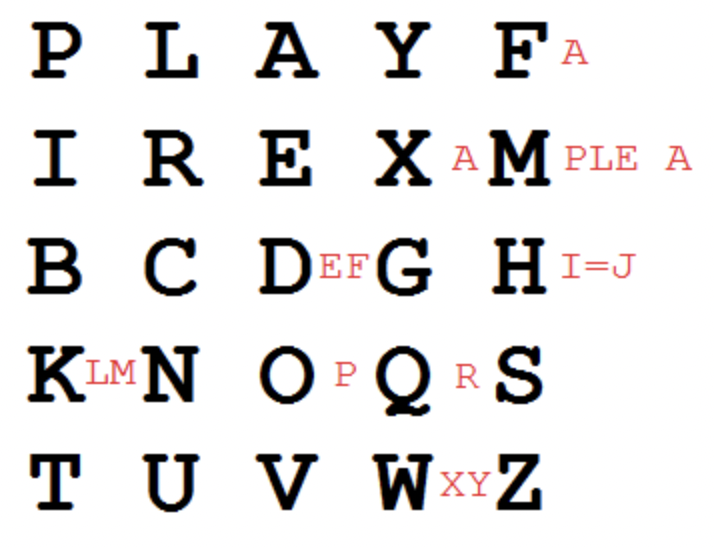
\includegraphics[scale=0.5]{playfair}
\end{center}
Il cyphertext è creato a coppia di lettere, si forma un rettangolo/quadrato utilizzando i vertici opposti delle due lettere scelte. I vertici opposti rappresentano le lettere cifrate.
\begin{figure} [H]
\begin{center}
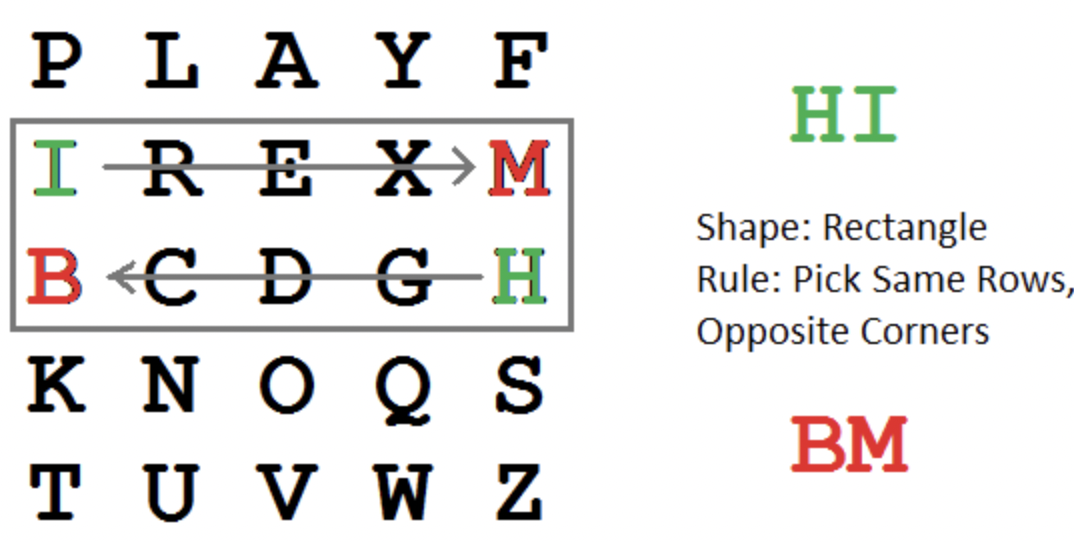
\includegraphics[scale=0.5]{playfair2}
\caption{I vertici opposti del rettangolo delle lettere HI sono BM, la codifica è BM}
\end{center}
\end{figure}
\noindent \textbf{Hill cipher}\\
Viene definita una matrice \emph{k} di dimensione \emph{n * n}, le parole vengono cifrate a coppie di n (matrice 2 x 2, cifrate 2 alla volta, matrice 3 x 3, cifrate 3 alla volta).\\
Un esempio può essere quella di prendere 2 lettere alla volta, codificate in numero, valore che è poi utilizzato per fare la moltiplicazione riga per colonna, il valore è passato a mod(26) per ricavare una lettera. Per decodificare facciamo la moltiplicazione per l'inverso della matrice chiave.\\
Non tutte le matrici chiavi sono ammissibili, la matrice deve esser invertibile per permettere il decifraggio da parte del destinatario. In particolare \(MCD(\Delta, 26) = 1\).\\\\
\textbf{ADFGX cipher}
Utilizzata dai generali tedeschi durante la prima guerra mondiale, viene creata una matrice 5 x 5 in cui vengono inserite le lettere arbitrariamente.
\begin{figure}[H]
\begin{subfigure}[h]{0.4\linewidth}
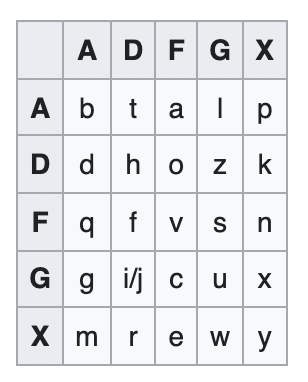
\includegraphics[width=\linewidth]{adfgx}
\end{subfigure}
\hfill
\begin{subfigure}[h]{0.6\linewidth}
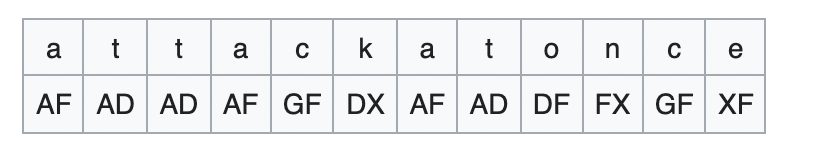
\includegraphics[width=\linewidth]{word}
\end{subfigure}%
\end{figure}
Per ricavare il crittotesto prendiamo le coppie degli indici (riga, colonna), ogni lettera quindi è data da una coppia di indici. \\Viene poi riordinato il crittotesto secondo una chiave di lunghezza k. Il crittotesto viene suddiviso in righe di k lunghezza. Una volta messe in pila di lunghezza k, le colonne vengono riordinate secondo l'ordine alfabetico delle lettere chiave.
\begin{figure}[H]
\begin{subfigure}[h]{0.2\linewidth}
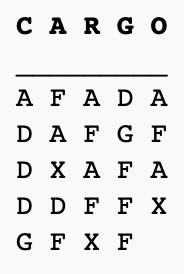
\includegraphics[width=\linewidth]{pre}
\end{subfigure}
\hfill
\begin{subfigure}[h]{0.5\linewidth}
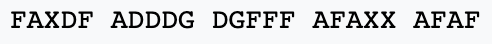
\includegraphics[width=\linewidth]{adfgx2}
\caption*{La codifica di CARGO}
\end{subfigure}
\hfill
\begin{subfigure}[h]{0.2\linewidth}
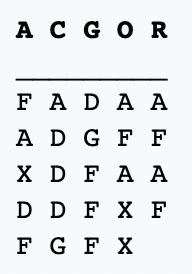
\includegraphics[width=\linewidth]{post}
\end{subfigure}%
\end{figure}
Con questo abbiamo finito con i cifrari storici.\\\\
\section*{NIST / NBS}
Il NIST è un'associazione governativa americata che si occupa di emettere bandi per richiedere la creazione di cifrari per il pubblico. In questo momento i bandi aperti sono: "Post-quantum competition" del 2018 ed il "Lightweight cryptography" per sistemi leggeri.\\
Nel 1970 manda un bando per creare un cifrario simmetrico utile alle grandi aziende americane per cifrare i dati sicuri, in particolare viene sviluppato DES, un cifrario simmetrico.
\section*{DES}
E' un cifrario a 16 round, basato su blocchi di 64, dotato di \emph{64 - 8 (bit di controllo) = 56} bit di chiave che produce un ciphertext di lunghezza 64. Un attacco di brute-forcing svolge al massimo $2^{56}$ tentativi, che già nel 1970 porta molti ad obbiettare.\\
Il plaintext è permutato per 16 volte, l'inverso della permutazione è poi applicato sul plaintext permutato.
\begin{figure}[H]
\begin{subfigure}[h]{0.4\linewidth}
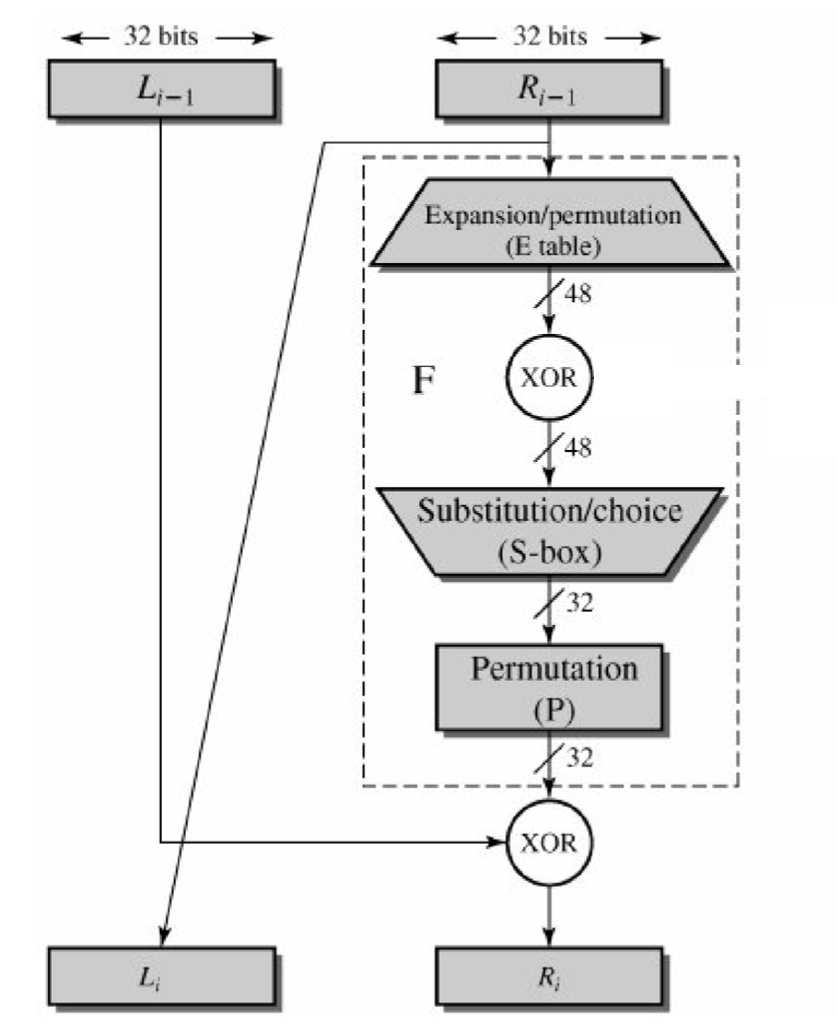
\includegraphics[width=\linewidth]{DES}
\caption*{F è la funzione di Feistel}
\end{subfigure}
\hfill
\begin{subfigure}[h]{0.4\linewidth}
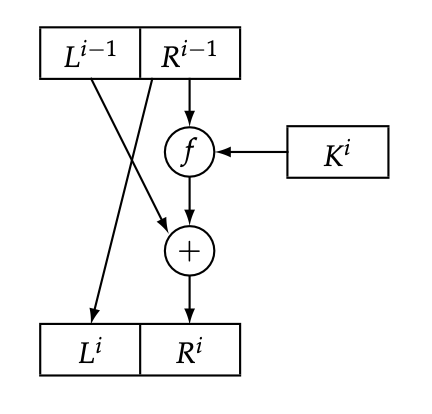
\includegraphics[width=\linewidth]{DES2}
\end{subfigure}%
\end{figure}
\section*{Feistel function}
\emph{Ma dove entra in gioco la chiave?} La chiave è fornita alla funzione di Feistel, è generata per ogni dato round di cifratura.\\\\
\emph{La funzione Feistel}\\
Quando parliamo di funzioni di Feistel parliamo di funzioni la cui sicurezza è acquisita effettuando \emph{n round} di permutazioni
\begin{center}
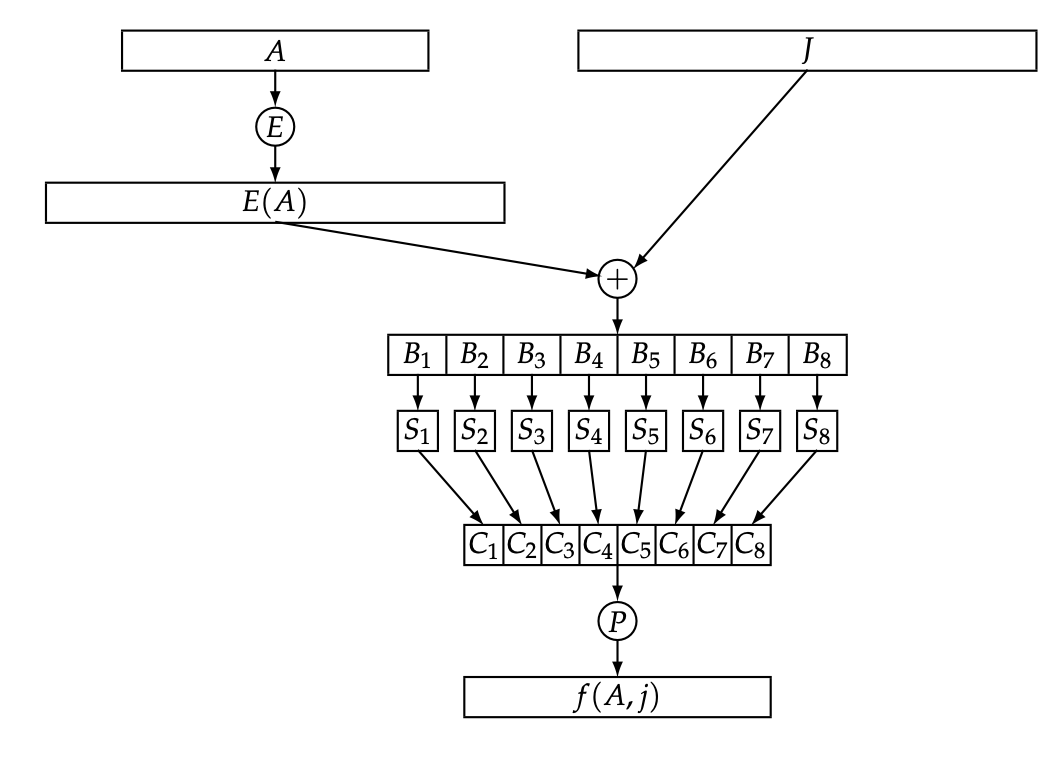
\includegraphics[scale= 0.4]{feistel}
\end{center}
La funzione \emph{E} è rappresenta permutazione di espansione, che aggiunge 8 bit ai 32 forniti in precedenza. Questi 48 bit 
sono utilizzati per effettuare uno XOR con \emph{J} (la chiave del round), che mi permette di ricavare 8 blocchi.
Questi 8 blocchi (formati da 6 bit ciascuno) sono permutati nuovamente (all'interno di $S_k$).
Le funzioni $S_k$ eseguono \emph{un'operazione di compressione}: prendono in bit 6 bit ciascuno, ma restituiscono 4 bit, portando l'output a 32 bit. Questi 32 bit rappresentano l'output.
\section*{S-Box}
La S-Box è un componente di compressione, $S_k$ è formato da una matrice $(4 * 16)$ sulla quale sono inseriti una permutazione dei valori tra 1 a 16 (fissa).
\begin{center}
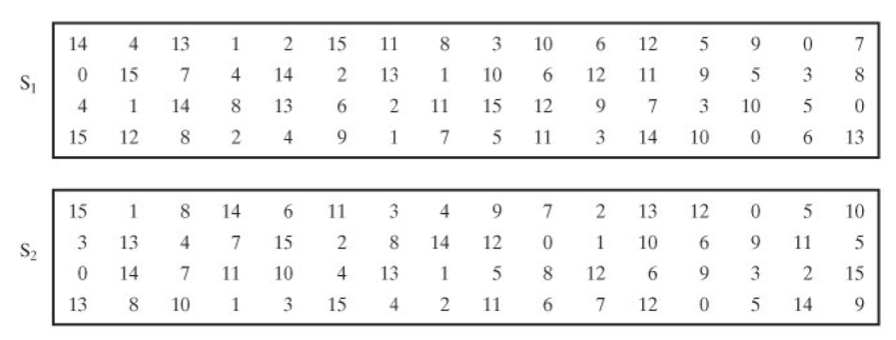
\includegraphics[scale= 0.7]{sbox}\\
\emph{un esempio di S-boxes}
\end{center}
Dato una sequenza di input di bit di lunghezza 6 (l'input di ogni s-box), il primo ed l'ultimo valore sono utilizzati per indicizzare la riga, ed i 4 valori interni indicizzano la colonna.
\begin{center}
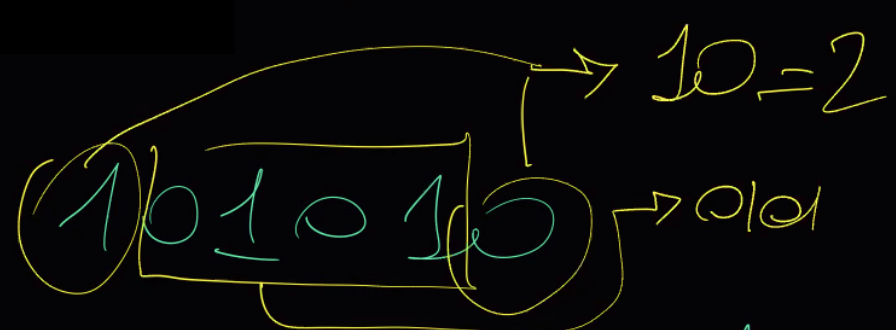
\includegraphics[scale= 0.8]{sbox1}\\
\emph{Si prende la terza e la sesta perché il binario 00 è la prima colonna, noi contiamo da 0}
\end{center}
Il valore ricavato incrociando riga e colonna codificato in binario rappresenta l'output della S-Box.
Questo è possibile perché nella matrice vi sono solo valori tra 0 e 15, che sono codificabili in binario su 4 valori.
\begin{center}
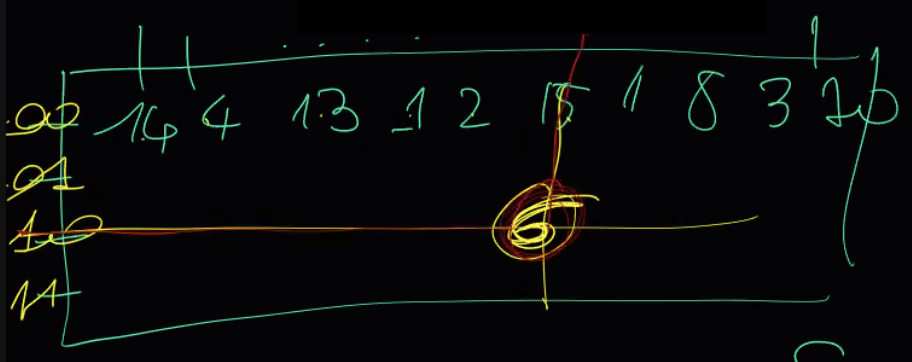
\includegraphics[scale= 0.8]{sbox2}\\
\emph{il valore di output di questa S-box sarà $0110_2$ = 6$_{(10)}$}
\end{center}
\section*{La chiave $K_i$}
\begin{center}
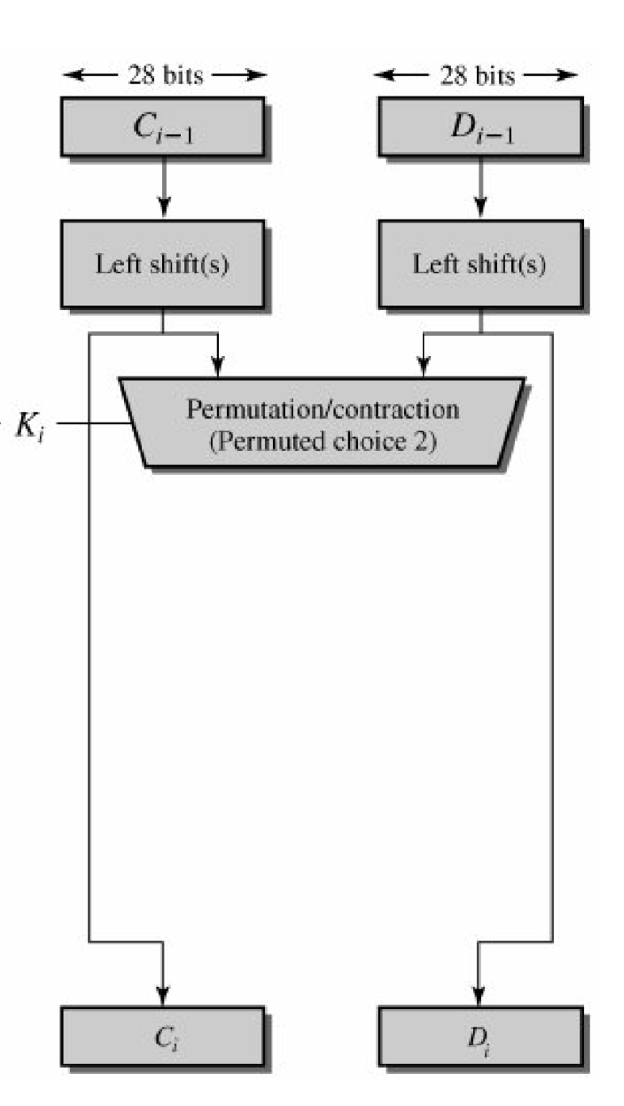
\includegraphics[scale= 0.6]{k1}
\end{center}
La chiave $K_i$ è formata da 64 bit, dalla quale vengono rimossi 8 bit di parità. Sui bit rimanenti è effettuata una permutazione. I 56 bit dopo la permutazione sono suddivisi in 2 blocchi da 28, chiamati rispettivamente $C_0$ e $D_0$. $C_0$ e $D_0$ sono shiftati a sinistra, a seconda del round.\\
$C_i$ = LS($C_{i-1}$)\\
$D_i$ = LS($D_{i-1}$)\\
Il valori shiftati vengono utilizzati come input per una permutazione/contrazione, passando da 56 a 48. L'output di questa permucontrazione rappresenta la chiave, e gli input della prossima $C_i$  e $D_i$.\\
\begin{center}
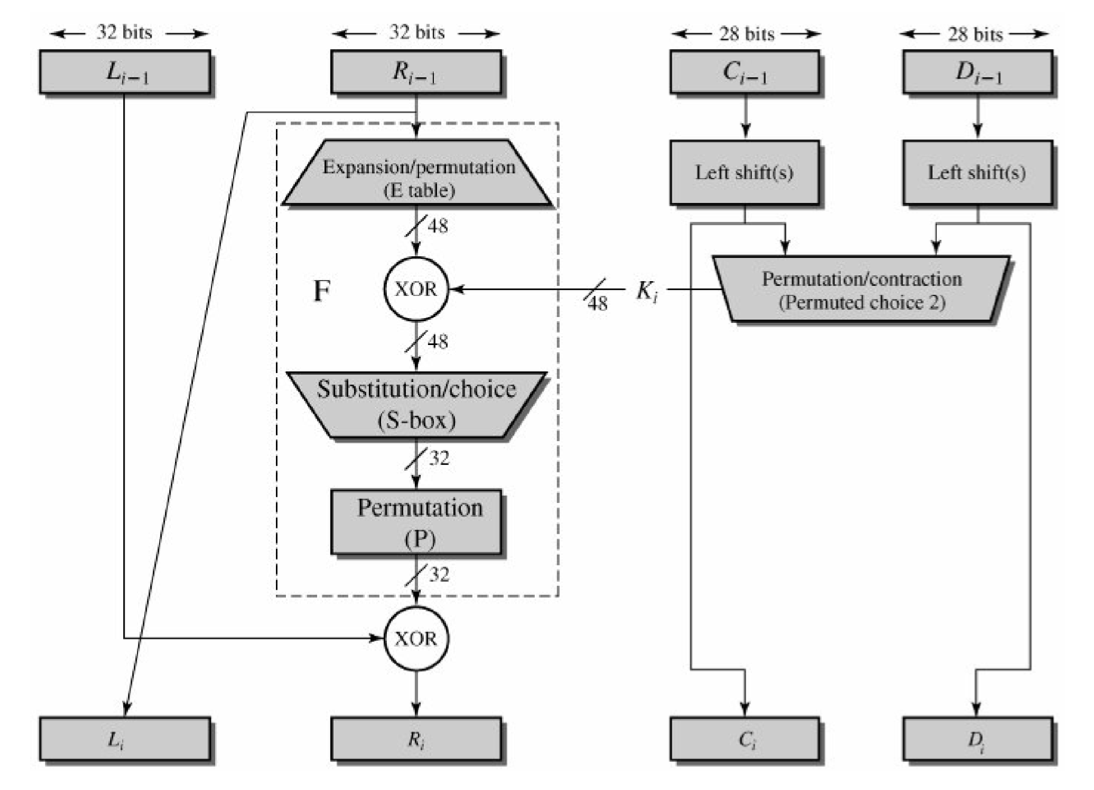
\includegraphics[scale= 0.5]{des3}\\
\emph{Overview di DES}
\end{center}
Vi sono dei vincoli riguardo a DES, per esempio:\\
E' importante che dato un S-Box, l'output di tale S-Box non possa in qualsiasi modo approssimabile.
\section*{S-DES | Simplified DES}
I dati:\\
\(plaintext = 12 bits \)\\
\(L_i = 6 bits\)\\
\(R_i = 6 bits\)\\
\(k = 9 bits\)\\
Il numero di round è diminuito, in particolare 3 (II, III, IV), tratteremo quindi:\\ \(L_1, R_1  \rightarrow L_2, R_2 = I° $ $  round\)\\ \(L_2, R_2  \rightarrow L_3, R_3 = II°  $ $round\)\\ \(L_3, R_3  \rightarrow L_4, R_4 = III° $ $ round\). \\\\
\emph{La funzione di Feistel semplificata:}\\
\(R_{(i-1)}\) (6 bits) è passato in espansione (8 bits), e fatta passata in XOR con la chiave (8 bits) (che perde un bit), per poi essere inserita come input (di 4 bits) in 2 S-Box di compressione (matrici 2 * 8).\\
L'output delle S-boxes sono di 3 bits ciascuna, il risultato è \(f(R_{i-1}, k_i\)).\\\\
\emph{La funzione di espansione E(x):}\\
La funzione di espansione ripete dei bit dell'input. In particolare dato un input:\begin{center}
(1-2-3-4-5-6) (6 bits), l'output sarà (1-2-4-3-4-3-5-6) (8 bits) \\in cui k rappresenta la posizione \(k_i\)\\
\end{center}
\emph{Le S-Box semplificate sono:}
\begin{center}
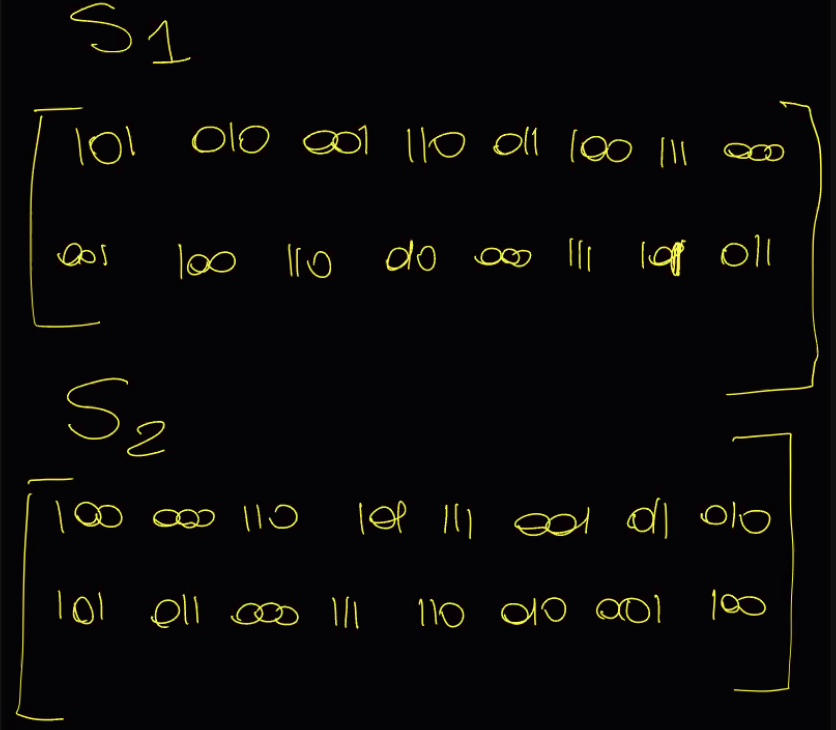
\includegraphics[scale= 0.5]{ssbox}\\
\end{center}
Per ricavare il valore di output è ricavato prendendo: il 1° bit per la riga, e gli altri 3 per la colonna\\
\emph{La compressione della chiave:}\\
La chiave è ricavata copiando la chiave a partire dalla posizione 2, ricopiando dall'inizio quando necessario.\\
\(k = 001001101\)\\
\(k_2 = 010011010\)\\
Il plaintext iniziale è: \(L_1R_1 = 000111-011011\) \\\\\

Il secondo plaintext è: \(L_1R_1 = 101110-011011\)\\
Qual'è \(L_4R_4?\)

L'operazione di crittoanalisi è eseguibile solo se il numero di round è basso (in particolare 3). Se i round sono 4, siamo sicuri che in mezzo c'è almeno un round di crittografia, se siamo a livello 5 sappiamo che sono almeno 2, e così via. L'attacco non è eseguibile deterministicamente, ma probabilisticamente.
\\\\
\emph{Le modalità di cifratura ECB, CBC, CFB, OFB, CTR}\\
Sono le modalità di utilizzo dei cifrari a blocchi, applicabili su qualsiasi cifrario a blocchi:
\begin{itemize}
\item ECB, o \emph{"electronic codebook mode"}:\\
ECB è applicato dividendo il plaintext P in blocchi di equa grandezza, che vengono poi codificati in cyphertext attraverso una cifrario a scelta. La dimensione del blocco è dipendente dal cifrario scelto\\
ECB è ideale quando la quantità di dati da codificare è bassa, se per esempio si vuole traasmettere una chiave DES, ECB è ideale.\\\\
Dato: \\$P = [p_1, ..., p_n]$ l'insieme delle porzioni di grandezza n\\
$C = [c_1, ..., c_n]$ l'insieme dei ciphertext di grandezza n\\
\emph{attraverso la funzione} $f(P_i; DES) = C_i$ possiamo codificare il plaintext in ciphertext 
Per ricavare il plaintext utilizziamo la funzione di decryption su ogni blocco di di ciphertext.
\begin{center}
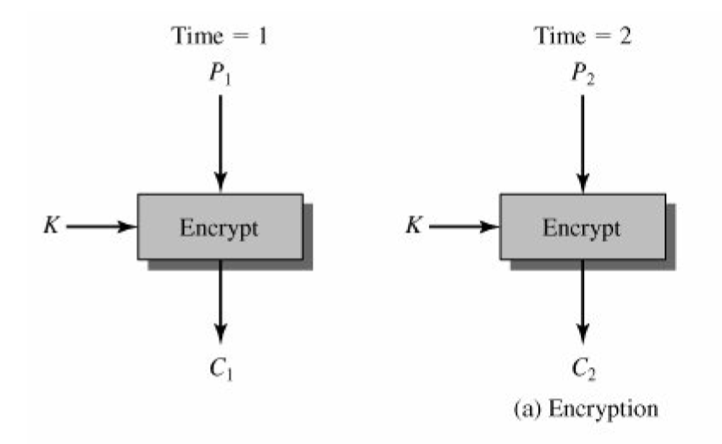
\includegraphics[scale= 0.7]{ecb}\\
\end{center}
Il problema con ECB è che se più blocchi di plaintext sono uguali, il ciphertext prodotto è uguale. Questo permette su messaggi molto lunghi di essere attaccati attraverso una crittoanalisi di frequenza
\item CBC, o \emph{"cipher block chaining mode"}:\\
Per mitigare le falle di sicurezza di ECB, vogliamo introdurre un meccanismo per produrre ciphertext differenti per plaintext diversi. Con CBC introduciamo un round di XOR con una chiave IV (Initialization vector)(pubblica o privata) prima della fase di encryption, per offuscare ulteriormente la procedura. IV è sostituito dal ciphertext del round $P_i-1$ dalla fase 2 in poi.
\begin{center}
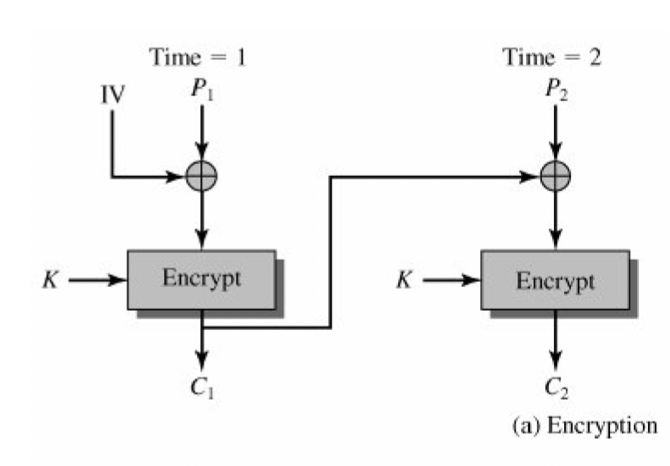
\includegraphics[scale= 0.7]{cbc}\\
\end{center}
Introduciamo una chiave \emph{IV} da applicare in XOR con la prima fase di encryption. Dalla seconda fase in poi l'IV è sostituito con il ciphertext del round $P_i-1$.
\end{itemize}
Il problema con queste modalità è che l'operazione di cifratura avviene su singoli blocchi, piuttosto che su singoli caratteri. Sarebbe comodo poter trasmettere singoli blocchi cifrati alla volta
\begin{itemize}
\item CFB, o \emph{"cipher feedback mode"}:\\
In questo schema di encryption, il vettore di inizializzazione è encryptato con la chiave $k$. $n$ bits dell'output sono utilizzati come input per un'operazione di XOR con il plaintext. L'output è inserito in coda al vettore di inizializzazione prossimo, shiftando l'IV precedente.
\begin{center}
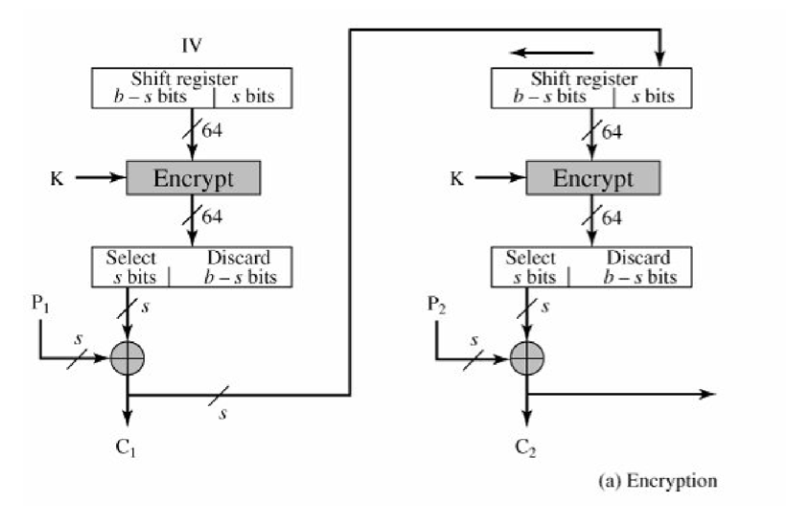
\includegraphics[scale= 0.7]{cfb}\\
\emph{da notare che l'output di encrypt sono 64 bit. \\si prende il primo blocco e quindi un char (8bits)}
\end{center}
In questa modalità la grandezza dei blocchi del plaintext è $s$ (di Select s-bits). \\Se $s = 1 char (8 bits)$, i blocchi del plaintext sono grandi $s$. \\
Il problema con questa modalità è che se compare un errore di trasmissione, esso si propaga, fintanto che il blocco corrotto venga espulso dall'IV.
\item OFB, o \emph{"output feedback mode"}:\\
Questo schema di encryption è molto simile a CFB, ma che risolve il problema di propagazione di errore di trasmissione. Il feedback, che in CFB proveniva dopo allo XOR con il plaintext, viene piuttosto estratto in locale, prima dello XOR.
\begin{center}
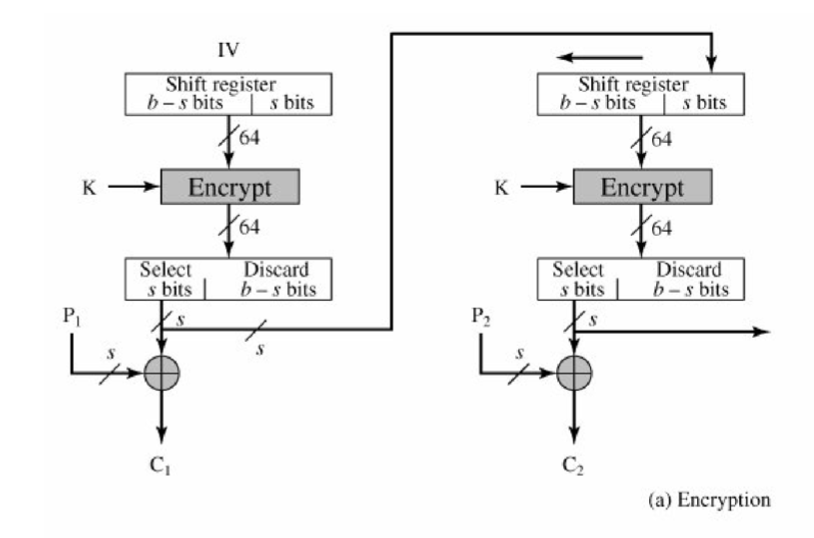
\includegraphics[scale= 0.7]{ofb}\\
\end{center}
Il problema con questa modalità è che le operazioni avvengono necessariamente sequenzialmente, piuttosto che in parallelo. 
\item CTR, o \emph{"counter mode"}:\\
Viene introdotto un counter che ha grandezza uguale al plaintext (che tuttavia deve essere necessariamente diverso rispetto ad ogni plaintext che si vuole encryptare). Le due parti devono concordarsi sul valore del counter iniziale, ma siccome il valore del counter è deterministico ed indipendente l'uno dall'altro, possiamo parallelizzare le operazioni di encryption.
\begin{center}
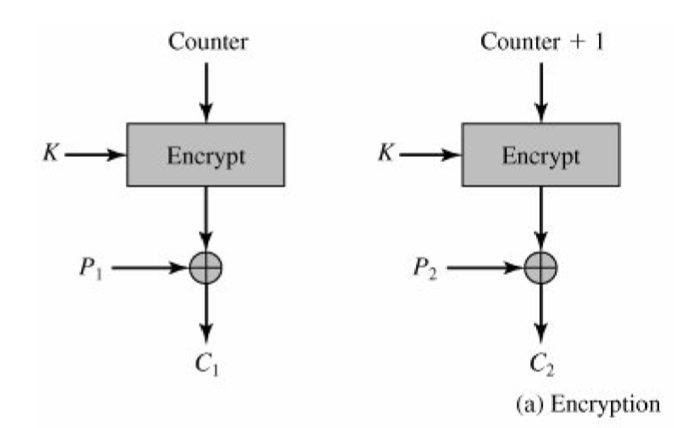
\includegraphics[scale= 0.7]{ctr}\\
\end{center}
\item XTS, o \emph{XEX-based tweaked-codebook mode with ciphertext stealing}\\
Modalità di cifratura applicata su dischi. \\Non possiamo utilizzare $2^{256}$ perché 256 non è un numero primo. E' basato su un polinomio irriducibile di grado 8 sul campo di Galois che ha grado massimo 7, ovvero\begin{center}
 $GF(2^8)$ : $ax^7+bx^6+cx^5+dx^4+ex^3+fx^2+gx^1+ h$ (range dei byte)
 \end{center}
Il polinomio $m(x) = ax^8+bx^7+cx^6+dx^5+ex^4+fx^3+gx^2+ hx^1 + i$ funge da modulo. Il grado è 8 perché quando andiamo ad effettuare il modulo, il risultato sarà sicuramente di grado $<$ $8$ che rientra ancora nel campo di Galois. I termini $a,b,...,i$ appartengono a $Z_2$ (0, 1)\\\\
Consideriamo $(x^7+1)x^7 = x^{14} + x^7$, come possiamo vedere il risultato sfora oltre il range dei byte gestiti.
Come nel cifrario di cesare effettuiamo un modulo, rispetto ad un polinomio $m(x)$ di grado 8
\begin{center}
$x^{14} + x^7 mod(m(x))$
\end{center}
\emph{Ma quale m(x) dobbiamo utilizzare?} \\Selezioniamo un $m(x)$ di grado 8 irriducibile (sono circa 30), ad esempio: \\$m(x) = x^8 + x^4 + x^3 +x+1$\\
Questo polinomio irriducibile è quello che è stato selezionato per AES.\\
Consideriamo $m(x)$, la sua scomposizione è: \\$m(x) * q(x) + r(x)$, e sul campo di Galois la rappresentazione di $m(x)$ è $r(x)$ \\\\
\emph{Cosa succede se ad AES applichiamo un polinomio $m'(x)$, ovvero un altro polinomio di grado 8 irriducibile ?}\\
In questo caso otterremmo un $r'(x)$, ovvero una rappresentazione diversa di $m(x)$

\end{itemize}
\emph{Double-DES | Doppio-DES}\\
Consideriamo un ciphertext cifrato con 2 round di DES, prima con una chiave $k_1$ e poi con una chiave $k_2$. Lo sforzo computazionale per decryptare il ciphertext richiederebbe $2^{56} + 2^{56}$ tentativi ovvero $2^{57}$, rispettivamente per ogni round.
\begin{center}
$C= E(k_2;E(k_1;p))$
\end{center}
\emph{Esiste una chiave $k_3$ che possa passare direttamente da plaintext a ciphertext?}\\
 - La risposta è no\\
 Il problema con questa implementazione è che le chiavi da mantenere diventano 2: $k_1, k_2$. Per arginare questo problema la funzione di encryption diventa:
 \begin{center}
 $C = E_{k_1}(D_{k_2}(E_{k_1}(plaintext)))$\\
 \emph{Ove $E$ è l'operazione di encryption, mentre $D$ è l'operazione di decryption}
 \end{center}
 Questa tecnica è chiamata \emph{Triple-DES o 3-DES} ed è il meccanismo alla base dei pagamenti elettronici. La decryption è effettuata con la chiave $k_2$, che però è diversa dalla chiave $k_1$, aggiungendo ulteriormente entropia.\\Se $k_1 == k_2$ l'operazione di encryption è svolta una sola volta (single DES), che ci permette di comunicare anche con dispositivi datati che non supportano l'encryption basato su più chiavi.
 
 
\section*{AES | Rijndael cipher}
Nel 1997 il NIST indice un nuovo contest per determinare un successore a DES, che verrà chiamato AES. Questo è fatto perché DES, avendo una chiave di 56-bit, era diventato vulnerabile ad attacchi brute force.\\
I 5 cifrari concorrenti arrivati alla finale sono: \emph{Rijndael, Serpent, Twofish, RC6, MARS}, Rijndael è selezionato nel 2001 in base a test di performance, efficienza su hardware datato, e supporto a chiavi di grandezza superiore e variabile.\\\\
In particolare AES:
\begin{itemize}
\item il plaintext ha blocchi di grandezza fissa 128 bits
\item la chiave a grandezza variabile: 128, 192 e 256 bits
\item il ciphertext ha grandezza 128 bits
\end{itemize}
\begin{center}
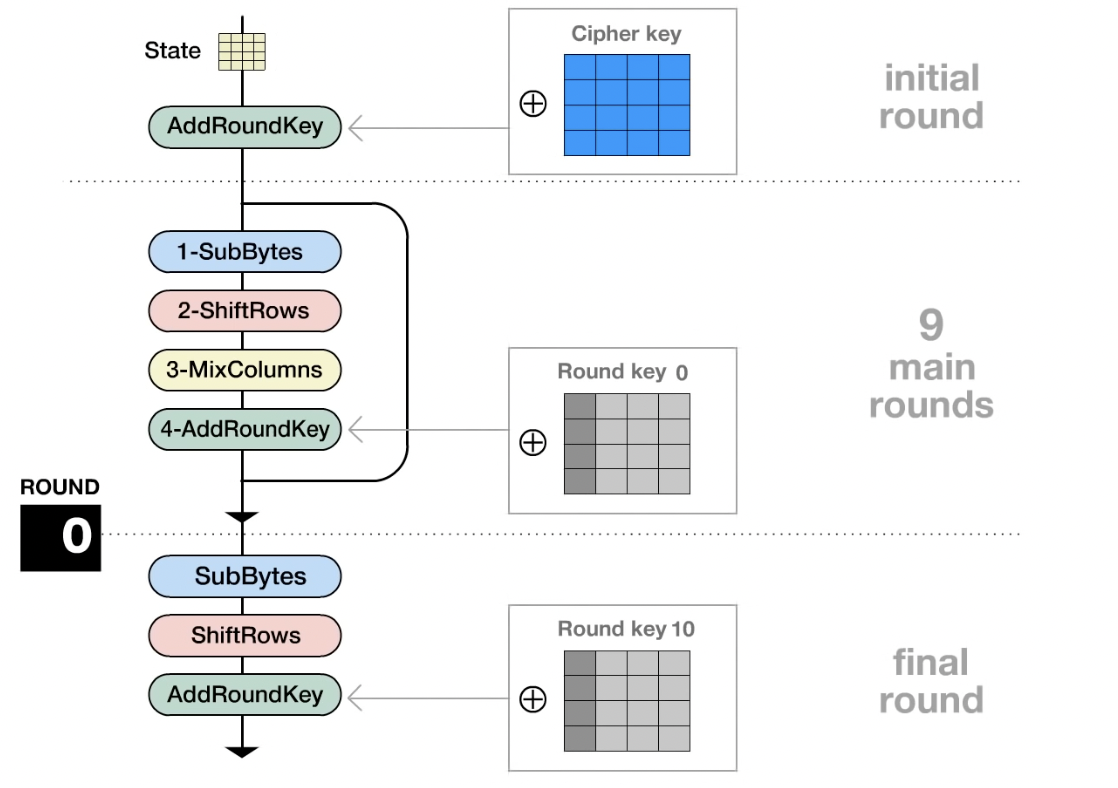
\includegraphics[scale= 0.4]{AES}
\end{center}
\emph{Add-round key}\\
E' l'operazione di "whitening" e ha l'obiettivo di neutralizzare il potenziale attacco basato su plaintext particolari (tutti 0, tutti 1 etc), consiste in un'operazione di XOR con la chiave colonna per colonna.\\\\
\emph{$Round_n$}\\
Le operazioni all'interno del $round_n$ sono svolte 9 volte e sono:
\begin{itemize}
\item Substitute bytes: corrisponde alle s-box in DES. in base ai valori presenti nello stato, vengono presi i valori all'interno di una matrice. Le s-box in AES sono di dimensione $16 * 16$\\
\emph{Ma come vengono calcolati i valori da inserire all'interno dell's-box?}
\begin{center}
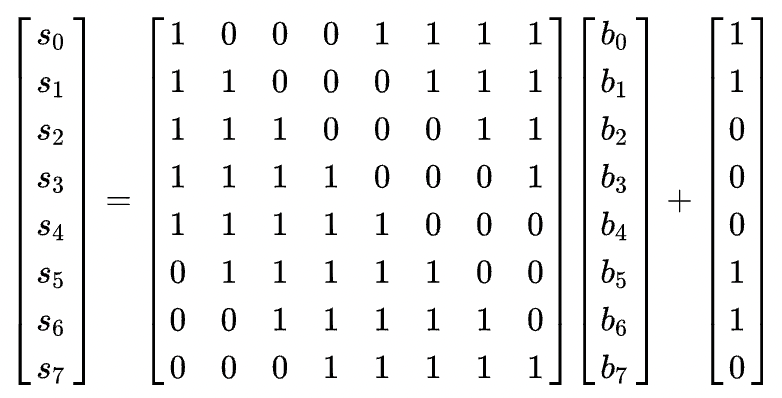
\includegraphics[scale= 0.4]{aesbox}
\end{center}
- Calcoliamo l'inverso moltiplicativo del valore $yx$ (ove. $riga = y$ e $colonna = x$) sul campo di Galois $GF(2^8)$\\
- Il byte risultante lo moltiplico per la matrice M\\
La matrice M è una matrice che è composta da n righe, costruite shiftando progressivamente verso destra il valore la seguente sequenza di bit: \begin{center}
1000 1111\\
1100 0111\\
...\\
fino a raggiungere\\
0001 1111
\end{center}
- Lo sommo per un valore costante C di valore 63\\
Il valore risultate è il valore da inserire all'interno della s-box in riga $y$ e colonna $x$.\\\\
Ricaviamo il valore a partire da 95:\\
- L'inverso moltiplicativo di 95  è $({95})^-1 = 8A$ \\
- Moltiplico l'inverso moltiplicativo per la matrice M (prodotto riga per colonna con la codifica in binario di $8A$)\\
- Faccio la somma con il valore 63 codificato in binario (11000110)\\
Il valore ricavato in riga 9, colonna 5 è 2A
\begin{center}
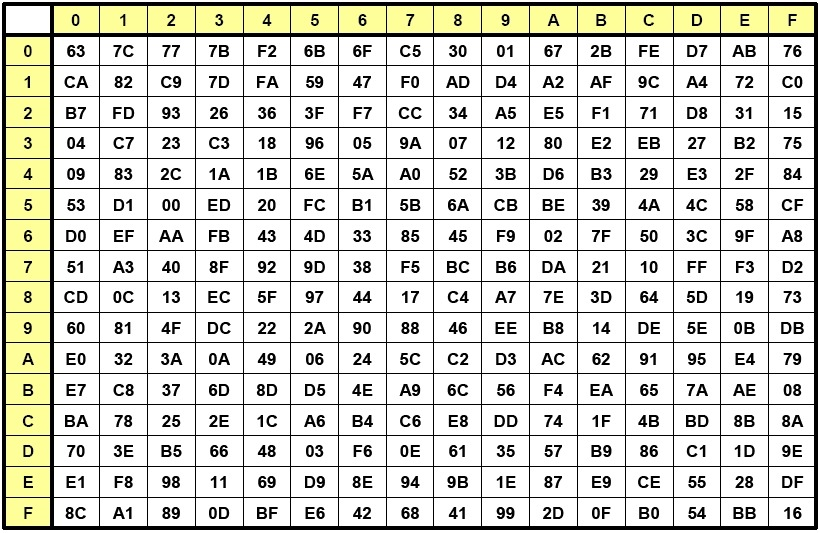
\includegraphics[scale= 0.3]{sbox3}
\end{center}
\item Shift rows: la prima riga viene lasciata invariata, la seconda viene shiftata di due byte, e la terza viene shiftata di 3 byte.
\item Mix columns: viene moltiplicata una colonna degli stati per una matrice nota, una colonna alla volta.
\item Add round key: un altro round di ARK, tuttavia 
\end{itemize}
\emph{$Round_9 + 1$ | $Round_{10}$}\\
Dopo aver svolto 9 volte le operazioni nel round, vengono effettuate nuovamente \emph{substitute bytes e shift rows}.\\
L'output del decimo round è il ciphertext.\\\\
\emph{Round keys | Key schedule}\\

\emph{AES-XTS}
\begin{center}
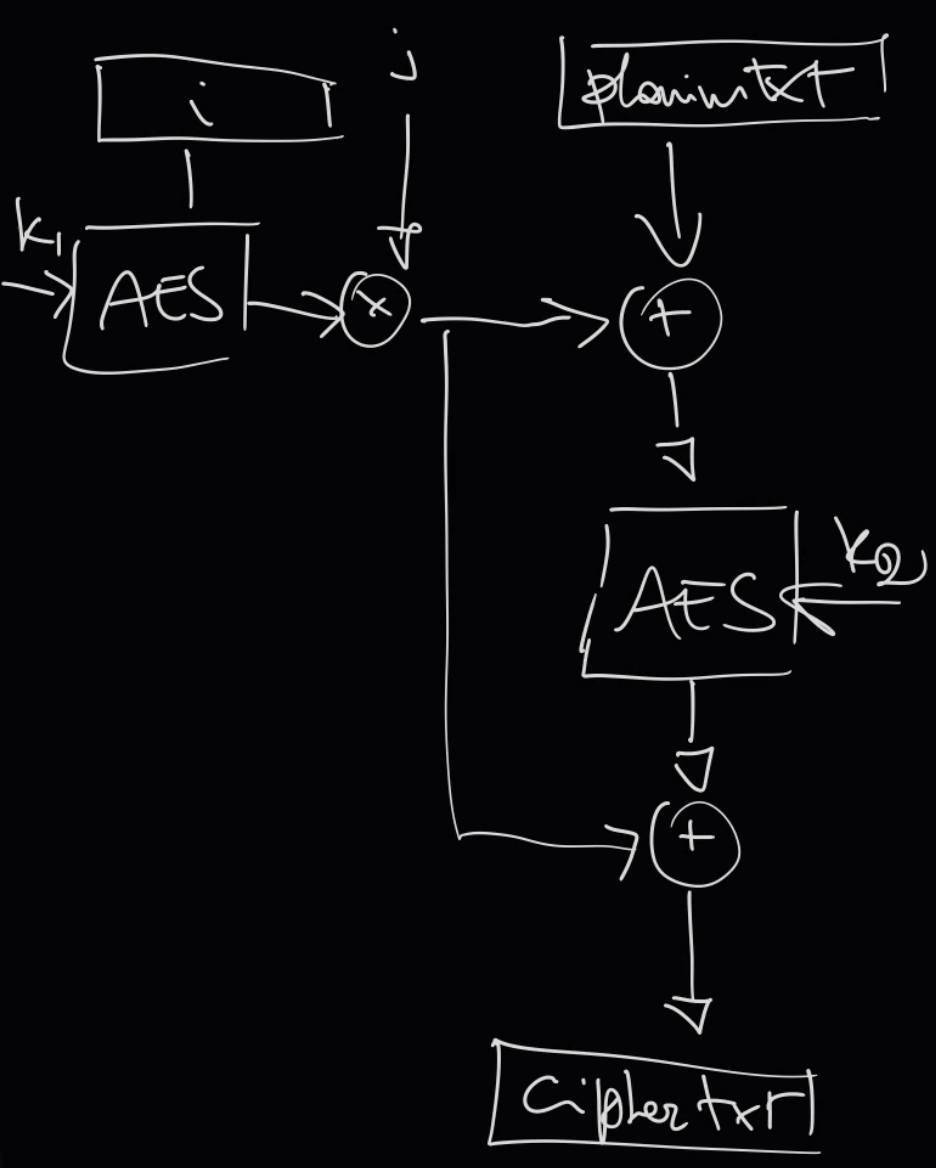
\includegraphics[scale= 0.4]{aesxts}\\
\end{center}
- AES $k_1$ e $k_2$ sono le due porzioni di chiavi di chiave AES applicate. $k_1$ e $k_2$ hanno dimensione 128, se la chiave AES ha 256 di dimensione. (Sono come il left and right)\\\\
- $i$ e $j$ sono rispettivamente il settore e la traccia del disco e hanno grandezza 128 bit. L'operazione che si svolge con $j$ è quella di prodotto (settore cifrato * traccia (non cifrata)). \\L'output è un polinomio in campo $GF(2^{128})$ con coefficienti su $Z_2$, con modulo $m(x) = x^{128}+x^7+x^2+x+1$\\
- Questo output è utilizzato per fare lo XOR con il plaintext, svolgendo un'operazione di whitening, prima di passare all'operazione di $AES_{k_2}$, passando per un whitening ulteriore abbiamo l'output.\\\\
Siccome i blocchi sono formati da 128 bit, è possibile che ci siano blocchi incompleti. In questi casi sono introdotti dei padding. \\Sia un plaintext diviso in blocchi $P_1, ... P_{m-1}, P_m$ con $P_m$ incompleto, in AES-XTS i blocchi  $P_1, ..., P_{m-2}$ sono gestiti normalmente, mentre i blocchi $P_{m-1}$ e $P_m$ sono gestiti in maniera speciale. In particolare:
\begin{itemize}
\item Il blocco $P_{m-1}$ è passato in AES-XTS, generando 
\begin{center}
$AES-XTS(<P_{m-1}>) = (C_{m}, CP)$
\end{center}
\item il blocco $P_{m}$ è incompleto, ed è complementato da un padding, in particolare n digits dal ciphertext $CP$ del blocco precedente.
\begin{center}
$AES-XTS(<P_m, CP_n>) = C_{m-1}$
\end{center}\end{itemize}
\begin{figure}[H]
\begin{subfigure}[h]{0.4\linewidth}
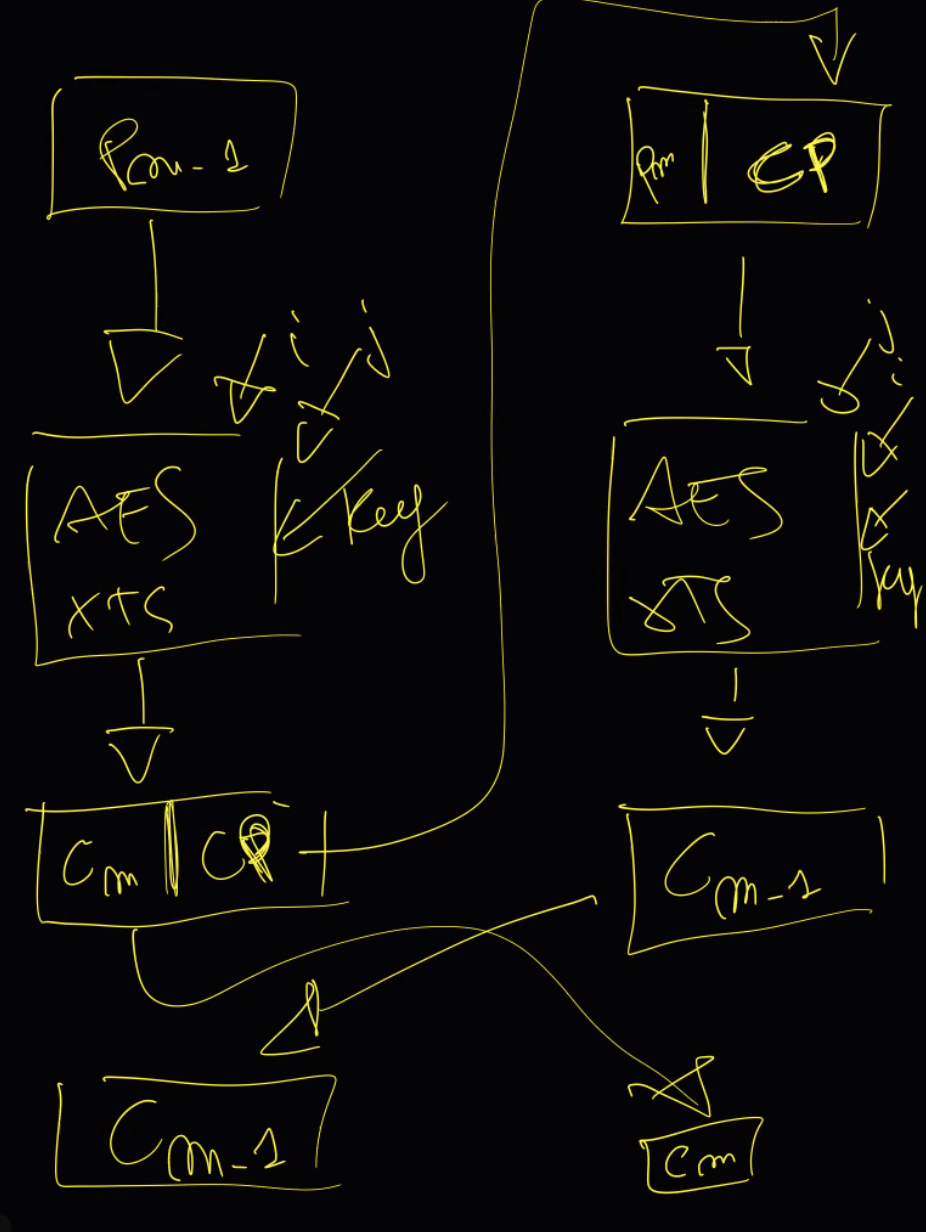
\includegraphics[width=\linewidth]{cpo}
\caption*{fase di encryption}
\end{subfigure}
\hfill
\begin{subfigure}[h]{0.4\linewidth}
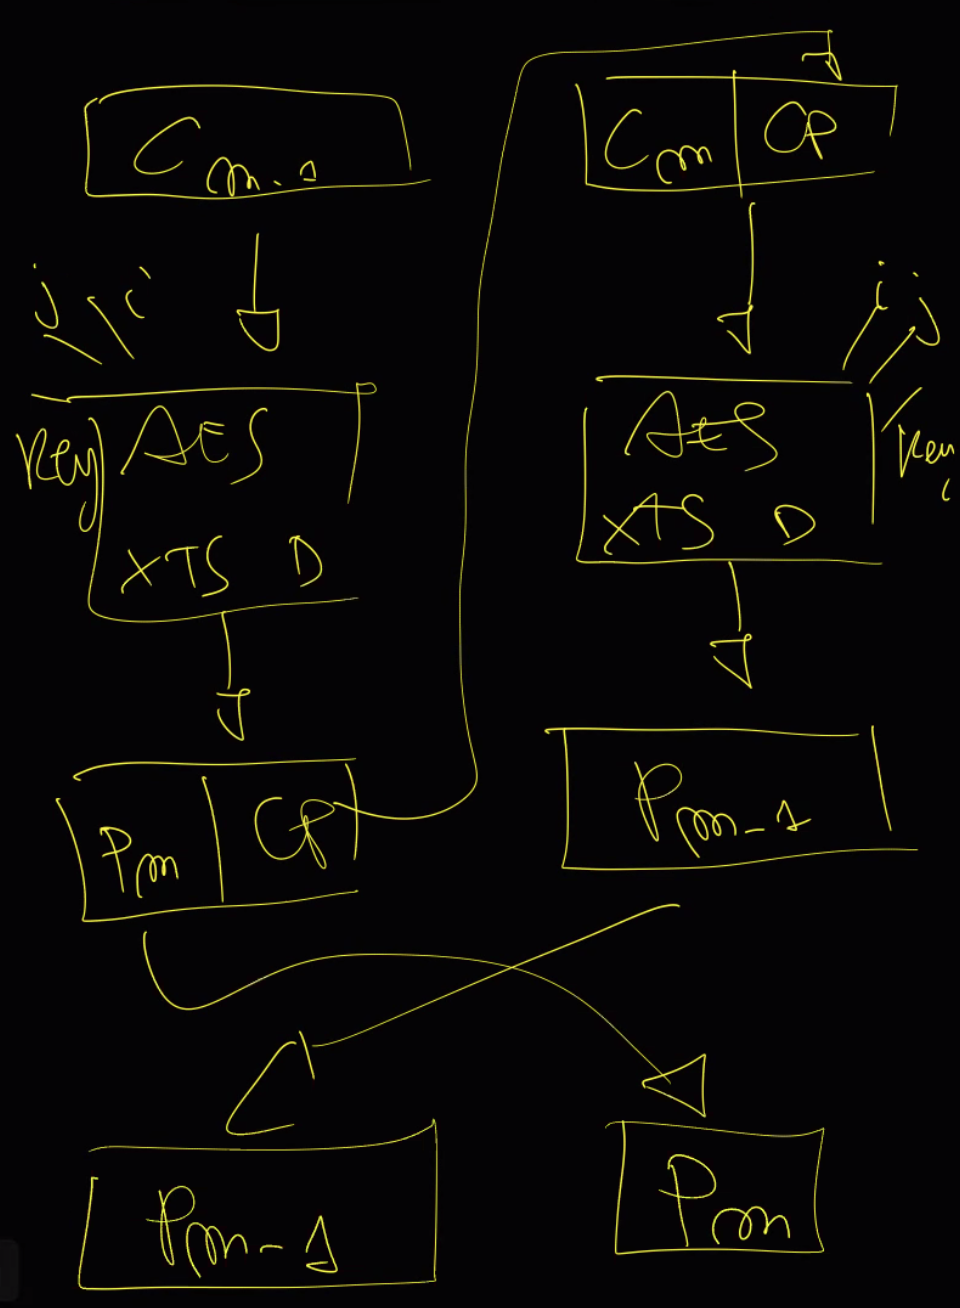
\includegraphics[width=\linewidth]{cpo-1}
\caption*{fase di decryption}
\end{subfigure}%
\end{figure}
La fase di decryption funziona al contrario (figure 2)

\section*{Attacking AES (6 rounds)}

\long\def\comment#1{
\emph{To be reviewed:  $https://www.davidwong.fr/blockbreakers/square_1_3rounds.html$}
}	
La prima cella all'interno della matrice 4x4 è designata e chiamata attiva, gli altri valori sono costanti.
$\Delta - SET$: l'insieme dei valori da 0 e 256 $P_1, ... P_{256}$ ovvero $00, 01, ... , FE, FF$\\
Somma zero (proprietà che ci permette di attaccare AES fino al terzo round): se prendiamo tutti i 256 crittotesti, lo xor su tutit i singoli byte in tutte le posizione la somma è uguale a 0, è una proprietà che vale fino al terzo round (dal round $\geq$ 4 non vale più \\
Le operazioni che vengono svolte sono in ordine : \emph{Add Round Key}, \emph{Substitute Bytes}, \emph{Shift Rows} ed infine \emph{Mix columns}. Possiamo tuttavia notare che le tutte le operazioni non vanno a modificare la posizione dell'active cell
\begin{center}
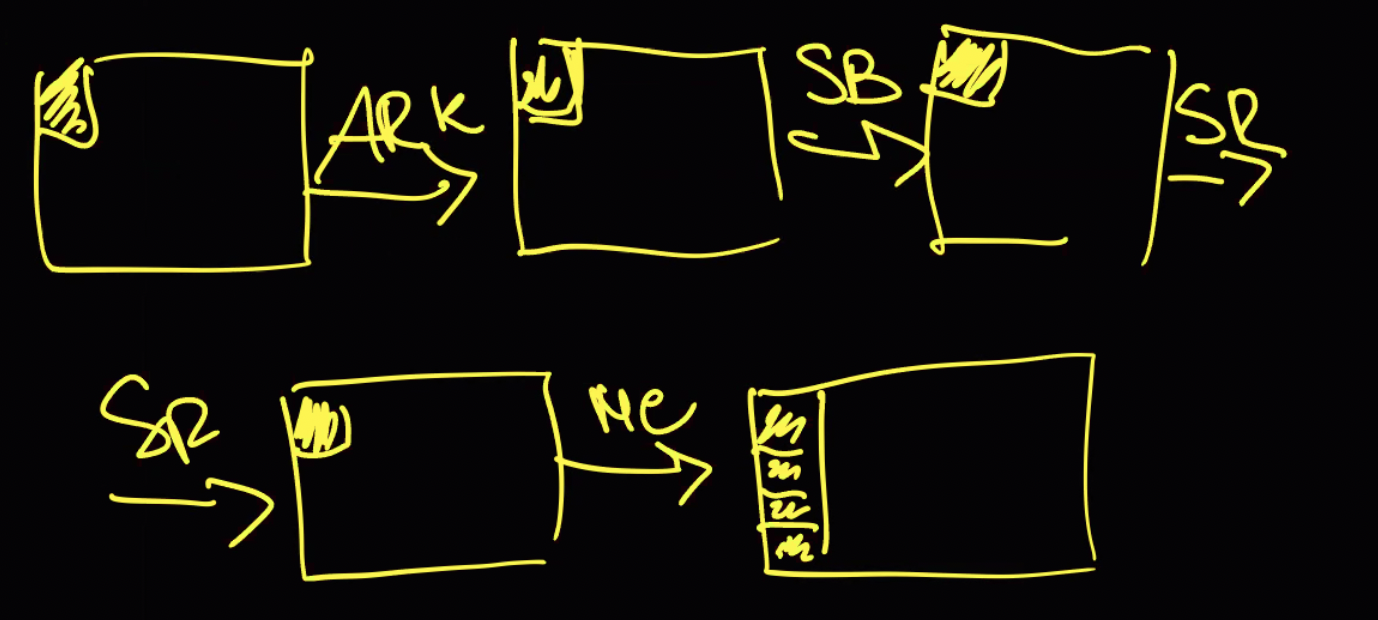
\includegraphics[scale= 0.4]{active}
\end{center}
Tuttavia, dal secondo round in poi, possiamo vedere che lo stato della cella attiva 1 va ad influire sul valore di tutte le altre.
\begin{center}
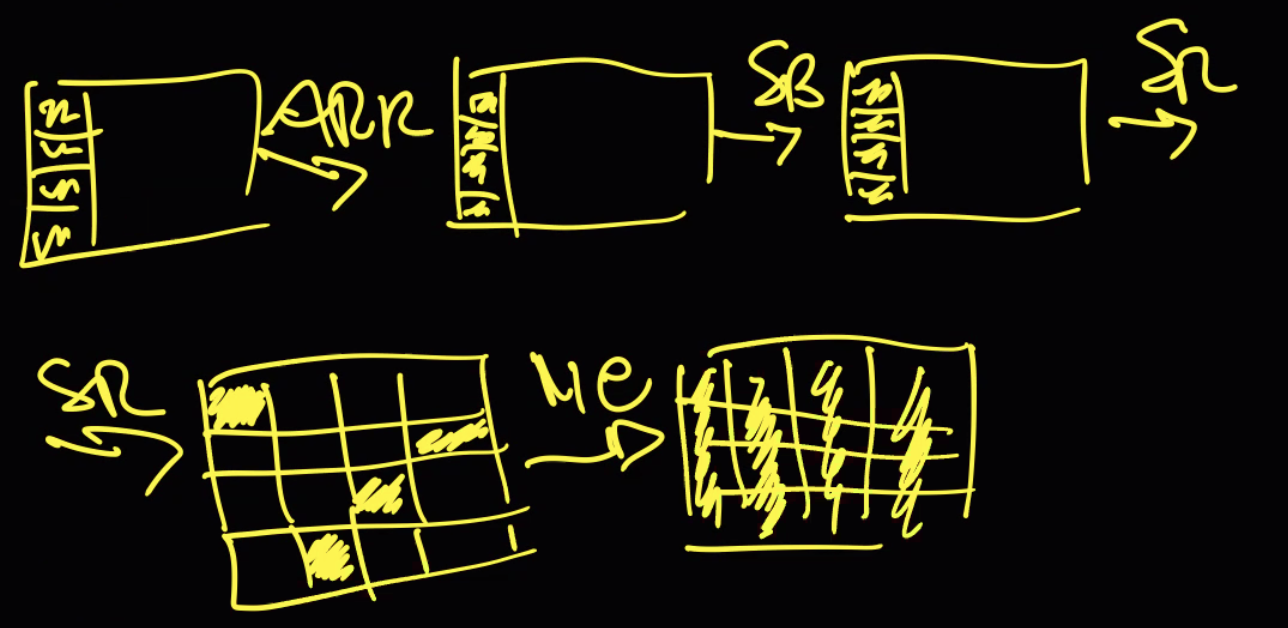
\includegraphics[scale= 0.4]{active2}\\
\end{center}
Una minima variazione del plaintext o della chiave va ad influire in maniera esponenziale sul ciphertext. Queste proprietà sono chiamate confusion and diffusion (tutto dipende da tutto). Un bit della chiave va ad influire tutto lo stato di AES\\\\\
$MC(stato)$ $\oplus$ $ARK$ = \\$MC(stato)$ $\oplus$ $MC(MC^{-1}(ARK))$ = \\$MC(stato$ $\oplus$ $MC^{-1}(ARK))$
\begin{figure}[H]
\begin{subfigure}[h]{0.5\linewidth}
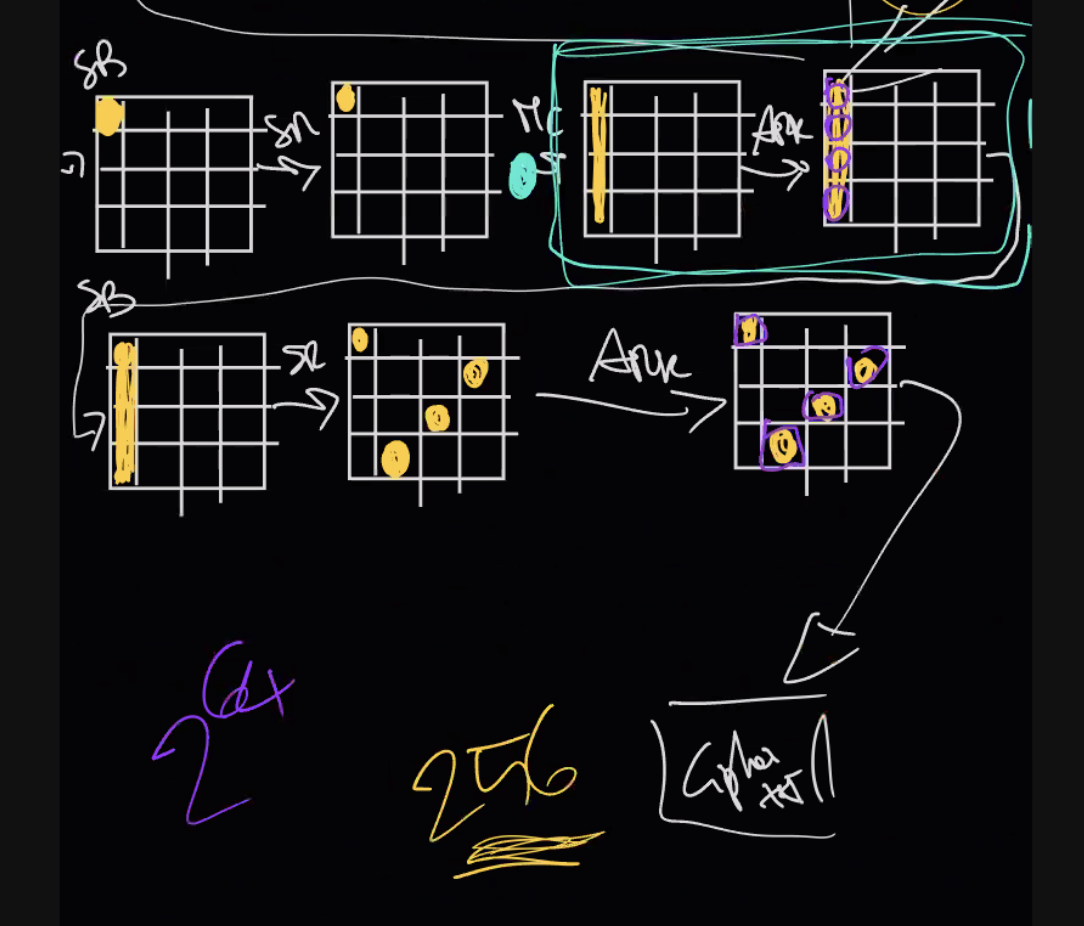
\includegraphics[width=\linewidth]{rev}
\end{subfigure}
\hfill
\begin{subfigure}[h]{0.5\linewidth}
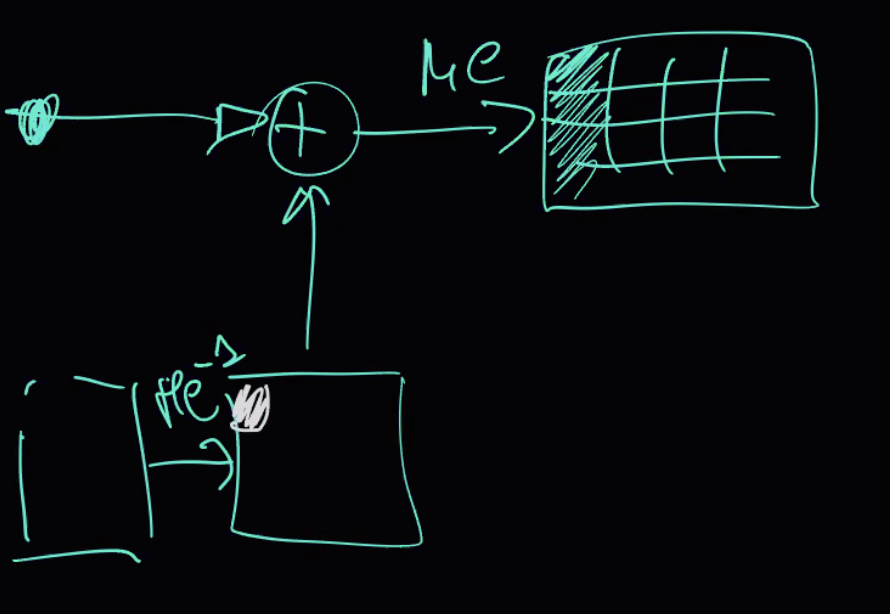
\includegraphics[width=\linewidth]{rev2}
\caption*{il pallino è la chiave, mi serve solo il primo byte della chiave}
\end{subfigure}%
\end{figure}
Lo sforzo computazionale è sceso da $2^{64}$ a $2^8* 5 = 2^{40}$, uno nel penultimo round, 4 nei round.
Per 5 round lo sforzo computazionale è $2^{32} * 2^{40} = 2^{72}$.
Guardare sullo stallings\\ \\

\section*{Crittografia asimmetrica}
Come abbiamo visto in precedenza, la crittografia asimmetrica differisce dalla crittografia simmetrica in quanto entrano in gioco più chiavi, le chiavi private. Le chiavi che entrano in gioco nei processi di cifratura e decifratura sono quindi differenti. \\Le chiavi nella crittografia asimmetrica sono di piccola grandezza, in quanto il mantenimento comporta uno sforzo computazionale non indifferente
\begin{center}
Encryption: $E_{pub}(M) = C$ \\
Decryption: $D_{priv}(C) = M$ 
\end{center}
Il processo di scambio di chiavi pubbliche avviene attraverso un processo di \emph{handshake}.
\subsection*{RSA}
E' un algoritmo di cifratura asimmetrica introdotto negli anni 70, il nome proviene dal nome degli inventori (Rivest-Shamir-Adleman). E' un cifrario a chiavi pubbliche, i principali soggetti sono:
\begin{itemize}
\item chiavi pubbliche: $public(n,e)$:\\
- (solitamente) $e = 2^{16}+1$\\
- $n = p * q$
\item chiavi private: $private(p,q,d)$:\\
- $p$ e $q$ sono due numeri (segreti) primi arbitraria grandi, in genere $>$ 1024 bit.\\
Questi valori devono essere grandi, per fornire un alto grado di entropia\\
- $d * e = 1$ $mod(\phi(n))$ (d segreto) \\
- $e$ è un numero casuale tale che $MCD(e, \phi(n)) = 1$
\end{itemize}

Le componenti pubbliche sono $n$ ed $e$, mentre le componenti private sono $p, d, e$\\\\
Alice: a fase di encryption avviene \begin{center}
$M^{e} = C$ $mod$ $n$ ove $M$  $<$ $n$
\end{center}
Bob: la fase di decryption avviene: \begin{center}
$C^d = M$ $mod$ $n$
\end{center}

\textbf{Il valore e}\\
Il valore $e$ è un valore casuale, che tuttavia deve essere scelto tale che valga la seguente condizione $MCD(e, \phi(n))=1$ (con l'applicazione dell'algoritmo di Euclide)\\ \emph{Ma perché viene scelto} $2^{16}+1$ \emph{solitamente?}\\
Consideriamo dove viene applicato: $m^e$ mod $n$, il valore $2^{16} = 65537$ in codifica binaria è: $10000000000000001$\\
Possiamo vedere che la compaiono molti 0, e pochi 1, ogni volta che compare 1 dobbiamo calcolare, quindi se minimizziamo il valore possiamo ridurre il numero di calcoli da effettuare. L'1 finale ci serve perché dobbiamo utilizzare un numero dispari. \\\\Il valore 65537 è scelto perché è un valore sufficientemente grande, che supera di un numero arbitrario di volte la $n$ nel modulo, aumentando lo sforzo computazionale richiesto al momento del calcolo della radice. In particolare quando andiamo a fare il bruteforcing, più grande è il valore $e$, più alto il valore che dobbiamo bruteforcare\\\\
\textbf{Il valore d}\\
Il valore $d$ è calcolato utilizzando l'algoritmo esteso di Euclide\\
\textbf{La fase di decryption ed encryption}\\
Viene utilizzato il $\phi(n)$\\

Per applicare l'algoritmo RSA abbiamo bisogno di un alcuni strumenti:
\subsection*{Coprimi: "l'algoritmo di Euclide" e "piccolo teorema di Fermat"}
Per verificare che due valori a, b siano coprimi, ovvero che $MCD(a, b)=1$ possiamo:
\begin{itemize}
\item Per valori non troppo grandi: per fattorizzare due valori a, b arbitrariamente grandi dobbiamo verificare tutti i numeri primi fino a radice di a. 
\item Per valori grandi utilizzare \emph{l'algoritmo di Euclide}
\end{itemize}
\textbf{L'algoritmo di Euclide per il calcolo dell'MCD}\\
L'algoritmo di Euclide è un algoritmo efficiente utilizzato per calcolare l'MCD di due valori interi. Se l'output dell'algoritmo di Euclide per due valori $a,b$ è 1 allora possiamo concludere che due valori sono coprimi.
\begin{center}
$a = bq_1 + r_1$\\
$b = r_1 q_2 + r_2$\\
$r_1 = r_2q_3 + r_3$\\
...\\
$r_{k-2} = r_{k-1}q_k+r_k$\\
$r_{k_-1} = r_kq_{k+1} + 0$\\
\end{center}
Se ci troviamo in questa situazione l'algoritmo di Euclide ha trovato resto uguale a 0.\\
L'MCD è quindi $MCD(a,b) = r_k$\\
Proviamo a fare il calcolo con $a = 1180, b= 482$
\begin{center}
$1180 = 482*  2 +216$\\
$482 = 216*2+50$\\
$216 =50*4+16$\\
$50=16*3+2$\\
$16=2*8+0$
\end{center}
Possiamo concludere che $l'MCD(1180, 482) = 2$\\\\
\textbf{L'algoritmo di Euclide esteso per l'inverso moltiplicativo}
\begin{center}
consideriamo $MCD(a,b) = ax+by$\\
\end{center}
\emph{Come calcoliamo x e y?}\\
Partiamo da x:\begin{center}
$x_0 = 0$\\
$x_1 = 1$\\
$x_2 = -q_{j-1} * x_1+x_0$\\
...\\
$x_j = -q_{j-1} * x_{j-1} + x_{j-2}$
\end{center}
Per calcolare y invece: \begin{center}
$y_0 = 1$\\
$y_1 = 0$\\
...\\
$y_j = -q_{j-1}*y_{j-1}+y_{j-2}$
\end{center}
Considerando $MCD(1180,482) = 2 = 1180y+482x$
\begin{center}
$x_0 = 0$\\
$x_1 = 1$\\
$x_2 = -2(1)+0 = -2$\\
$x_3 = -2(-2)+1= 5$\\
$x_4 = -4(5)-2 = -22$\\
$x_5 = -3(-22)+5 = 71$\\
Ricaviamo che $x = 71$\\
\end{center}
\begin{center}
$y_0 = 1$\\
$y_1 = 0$\\
$y_2 = -2(0)+1 = 1$\\
$y_3 = -2(1)+0= -2$\\
$y_4 = -4(-2)+1 = 9$\\
$y_5 = -3(9)-2 = -29$\\
Ricaviamo che $y=-29$
\end{center}
Allora abbiamo che $MCD(1180,482) = -29(1180) + 71(482) = 2$\\\\
L'inverso moltiplicativo deve essere $= 1$, ovvero $ax+by =MCD(a,b)=1$
Poniamo noi l'inverso moltiplicativo =1 perché il processo di decifratura è unica, se avessimo 2 ci sarebbero più decifrature possibili
\begin{center}
$by \equiv 1$ mod $a$\\
$by \equiv 1 + tot * a$ ove $tot = x$\\
$y*b = 1$ mod $a$
\end{center}


\textbf{Teorema piccolo di Fermat ed il teorema di Eulero}\\
Il teorema piccolo di Fermat dice che se $p$ è un valore primo, per ogni intero $a$, il valore $a^p-a$ è un intero multiplo di $p$.
\begin{center}
$a^p \equiv a$ $(mod$ $p )$  oppure  $a^{p-1}\equiv 1$ $(mod$ $p )$
\end{center}
Attraverso il \emph{teorema di Eulero} possiamo generalizzare il teorema di Fermat, in particolare: per ogni modulo $n$ ed ogni intero $a$ coprimo rispetto a $n$ abbiamo:
\begin{center}
$a^{\phi(n)} \equiv 1$ $(mod$ $n)$
\end{center}
Ove $\phi(n)$ rappresenta la funzione di Eulero, che conta il numero di interi fra 1 e $n$ coprimi rispetto ad n. Se $n = p$ è un numero primo allora 
\begin{center}
$\phi(p) = p-1$
\end{center}
Vediamo un esempio di applicazione del piccolo teorema di Fermat.\\
Supponiamo di voler calcolare $2^{43210}$ $mod$ $101$.
\begin{center}
Trasformiamo l'esponente: $43210$ in  $432*100 + 10$\\
$(2^{100})^{432}  * 2^{10}$ mod $101$\\ 
Teorema di Fermat: \\$a^{p-1}\equiv$ mod $p$\\
Allora $1^{432} * 2^{10} $ mod 101\\
Infine: $1024$ mod $101 = 14$
\end{center}
\subsection*{Attacking RSA}
Siccome il cifrario RSA è stato introdotto nel 1970, durante gli anni sono stati eseguiti numerosi attacchi, che vertono sulle problematiche algoritmiche, matematiche ed ingegneristiche. \\\\
\emph{$\phi$(n) accessibile}\\
Consideriamo un caso in cui l'attaccante sia in grado di accedere al valore $\phi(n)$, magari attraverso ad un dump della memoria dopo che un programmatore l'ha utilizzato, senza cancellare il valore. Siccome i valori della chiave pubblica sono $(n, e)$, abbiamo i seguenti valori disponibili: $(n, e, \phi)$. Se effettuiamo:
\begin{center}
$n-\phi(n)+1 =$\\
$=pq-[(p-1)(q-1)]+1=$\\
$=pq-[pq-p-q+1]+1=$\\
$=p+q$
\end{center}
Deduciamo che se troviamo $\phi$ possiamo ricavare $p+q$. \\Consideriamo ora che $n=p*q$
\begin{center}
$ax^2+bx+c$ \\ove $c = p*q = n$, $a =1$, $b = p+q$\\
$x_1x_2 = c/a$\\
$x_1+x_2 = -b/a$
\end{center}
Possiamo quindi ricavare che\begin{center}
$x^2-x(n-\phi(n)+1)+n=0$\\
Se risolviamo con il $\Delta$ possiamo ricavare i valori $x_1 = p $ e $x_2 = q$
\end{center}

Considerando:\begin{center}
$m^e = a$ mod$ $n$\\




\end{document}  